\subsection{Reasoning Efficiency and Control}
\label{subsec:reasoning_effort}

Nemotron 3 Ultra is trained for three reasoning modes: reasoning-off, regular and medium-effort. The regular and medium-effort reasoning modes have the option to be used in conjunction with inference-time budget control. These combinations of controls provide flexibilities that cover the entire spectrum of accuracy-efficiency trade-off to meet customers’ needs in various application scenarios and complement task-level controls such as turn-limits in agentic applications.

The medium-effort reasoning mode is introduced during the SFT stage and later optimized during the RLVR stage. Approximately 2.5\% of the RLVR training prompts are in the medium-effort mode and they cover math, STEM and coding, and length-based adjustments are applied on the RL rewards for them. This recipe has trained both Nemotron 3 Ultra and Super and the effects of optimization generalize to a variety of tasks beyond math, STEM and coding, and we were able to calibrate the resulting effort mode by adjusting hyperparameters.

Figure~\ref{fig:reason_effort} compares Nemotron 3 Ultra, Nemotron 3 Ultra medium-effort and Nemotron 3 Super against a set of open-source models. The y-axis is Artificial Analysis Intelligence Index V4 while the x-axis is a relative verbosity measure by using Qwen 3.5 397B's average token usage on each task as reference and by averaging over the 10 tasks in AA Index V4. It shows that Ultra's medium-effort mode uses on average around 2.5X less tokens than the regular mode at the cost of approximately 7\% drop in accuracy.

\begin{figure}[ht!]
    \centering
    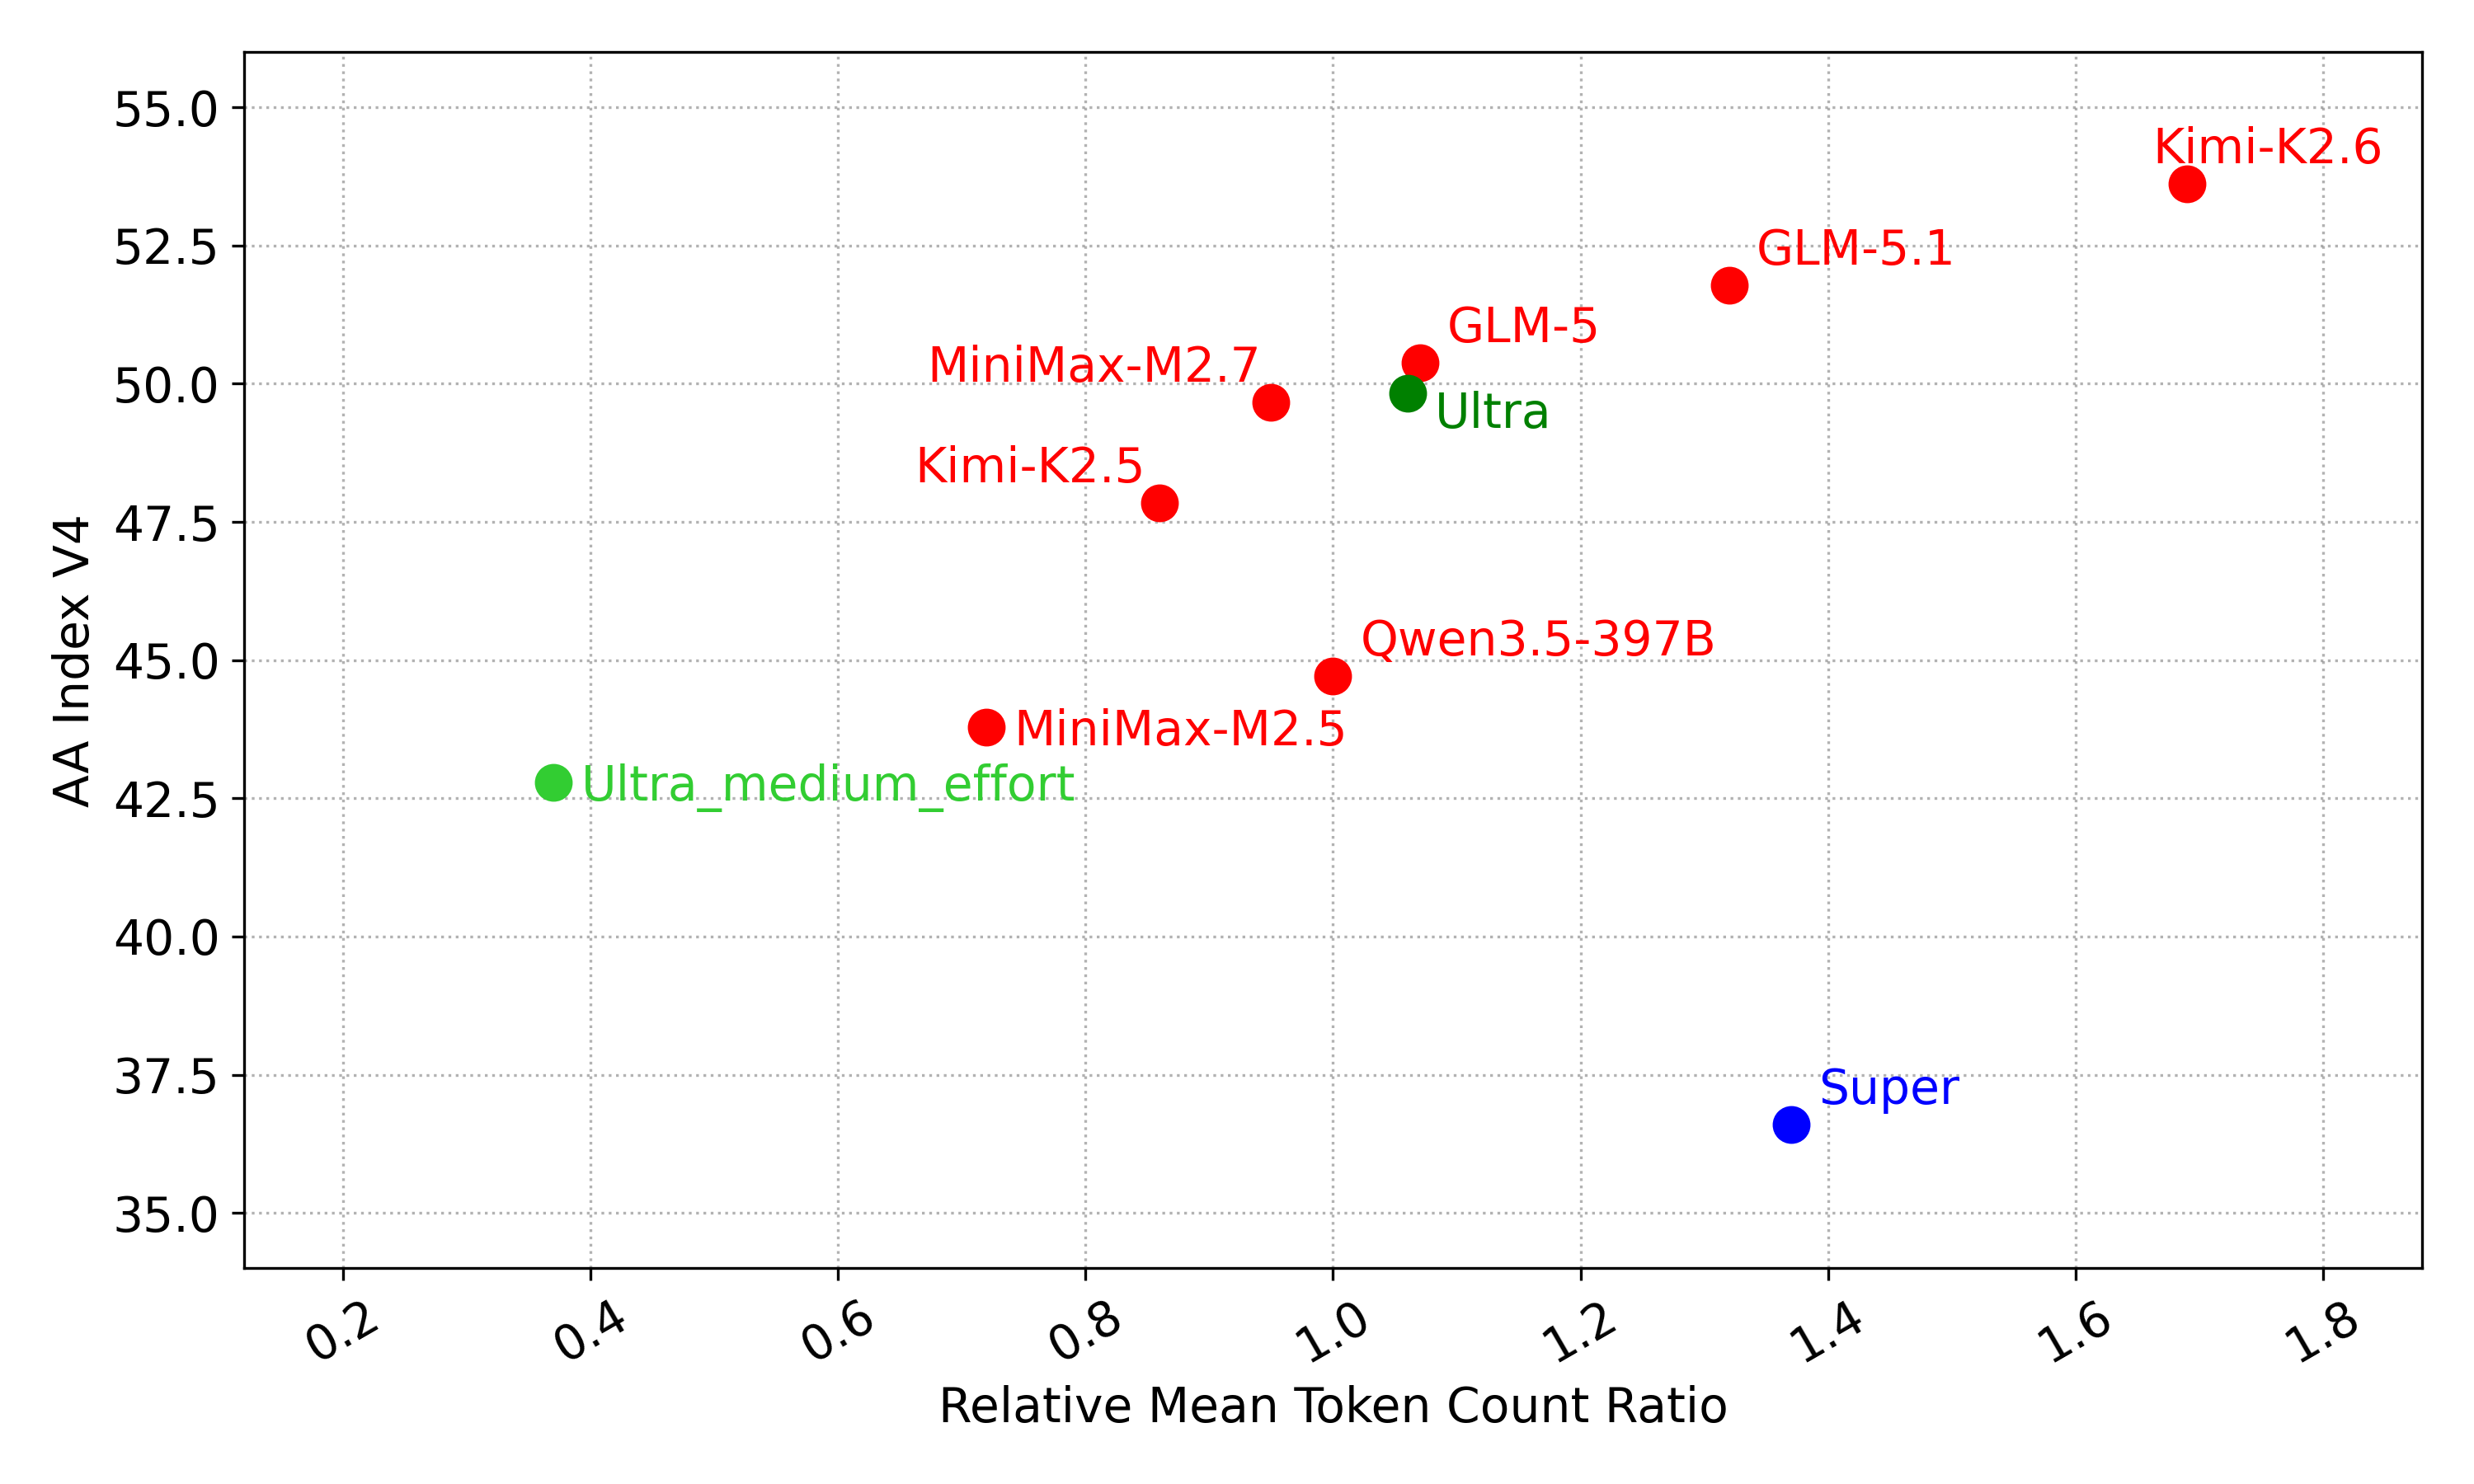
\includegraphics[width=0.9\linewidth]{figures/5_26_aa_mean_token_ratio_highreso.png}
    \vspace{-0.5em}
    \caption{Accuracy-efficiency comparisons on Artificial Analysis Intelligence Index V4 tasks.}
    \label{fig:reason_effort}
    \vspace{-0.5em}
\end{figure}
